\documentclass[12pt]{article}
\usepackage[english]{babel}
\usepackage[utf8x]{inputenc}
\usepackage{amsmath}
\usepackage{graphicx}
\usepackage{caption}
\usepackage{booktabs}
\usepackage{float}
\usepackage[colorinlistoftodos]{todonotes}
\usepackage{subcaption}
\usepackage[colorlinks=true, linkcolor=blue]{hyperref}
\usepackage{array}
\usepackage{makecell}
\usepackage[margin=1in]{geometry} % added: 1 in margins to fit the 15-page limit (remove to restore default margins)
\usepackage{tikz} % added for the block diagram
\usetikzlibrary{arrows.meta,positioning}
\newcommand{\rOneA}{55.1}
\newcommand{\srOneA}{2.5}
\newcommand{\rTwoA}{60.0}
\newcommand{\srTwoA}{2.6}
\newcommand{\NoneA}{496}
\newcommand{\NtwoA}{540}
\newcommand{\pSlope}{0.041}
\newcommand{\spSlope}{0.030}
\newcommand{\pPct}{7.4}
\newcommand{\spPct}{5.4}
\newcommand{\rEightThirty}{61.0}
\newcommand{\srEightThirty}{4.5}
\newcommand{\rEightFifty}{61.7}
\newcommand{\srEightFifty}{4.5}
\newcommand{\rNineTen}{89.0}
\newcommand{\srNineTen}{5.4}
\newcommand{\rSevenTen}{50.7}
\newcommand{\srSevenTen}{4.1}
\newcommand{\rSixSeventy}{14.7}
\newcommand{\srSixSeventy}{2.2}
\newcommand{\rSixNinety}{39.7}
\newcommand{\srSixNinety}{3.6}
\newcommand{\phRatio}{19}
\newcommand{\coV}{3.77}
\newcommand{\coRate}{147.3}
\newcommand{\scoRate}{2.2}
\newcommand{\coCh}{2906}
\newcommand{\coG}{4419}
\newcommand{\bkgR}{1.0}
\newcommand{\sbkgR}{0.45}
\newcommand{\grossA}{68.0}
\newcommand{\sgrossA}{3.7}
\newcommand{\netA}{67.0}
\newcommand{\snetA}{3.7}
\newcommand{\lnA}{4.20}
\newcommand{\slnA}{0.055}
\newcommand{\netB}{15.6}
\newcommand{\snetB}{1.9}
\newcommand{\lnRatio}{1.457}
\newcommand{\dtAB}{0.05186}
\newcommand{\nTwo}{28.1}
\newcommand{\snTwo}{4.5}
\newcommand{\nExp}{105}
\newcommand{\snExp}{10}
\newcommand{\nRatio}{3.7}
\newcommand{\EMeas}{0.74}
\newcommand{\sEMeas}{0.08}
\newcommand{\EExpFit}{0.31}
\newcommand{\EFig}{0.32}
\newcommand{\tailA}{11.6}
\newcommand{\stailA}{0.6}
\newcommand{\tailB}{5.5}
\newcommand{\stailB}{0.6}
\newcommand{\sMb}{0.5}
\newcommand{\sMone}{117.4}
\newcommand{\sMtwo}{44.6}
\newcommand{\sMonetwo}{158.5}
\newcommand{\sX}{5157}
\newcommand{\sY}{8.20\times10^{5}}
\newcommand{\sZ}{0.092}
\newcommand{\sTau}{298}
\newcommand{\ssTau}{566}
\newcommand{\tauMean}{627}
\newcommand{\tauSD}{337}
\newcommand{\tauSEM}{195}
\newcommand{\tauPool}{605}
\newcommand{\stauPool}{362}
\newcommand{\nSigScope}{1.4}
\newcommand{\limA}{2778}
\newcommand{\limB}{1022}
\newcommand{\sDead}{360}
\newcommand{\ssDead}{3}
\newcommand{\sInt}{480}
\newcommand{\sInit}{840}


\newcolumntype{C}[1]{>{\centering\arraybackslash}p{#1}}
\bibliographystyle{ieeetr}


\begin{document}

\begin{titlepage}

\newcommand{\HRule}{\rule{\linewidth}{0.5mm}} % Defines a new command for the horizontal lines, change thickness here

\center % Center everything on the page
 
%----------------------------------------------------------------------------------------
%	HEADING SECTIONS
%----------------------------------------------------------------------------------------

\textsc{\LARGE University of Michigan}\\[1.5cm] % Name of your university/college
\textsc{\Large NERS 515}\\[0.5cm] % Major heading such as course name
\textsc{\large Nuclear Measurements Laboratory}\\[0.5cm] % Minor heading such as course title

%----------------------------------------------------------------------------------------
%	TITLE SECTION
%----------------------------------------------------------------------------------------

\HRule \\[0.4cm]
{ \huge \bfseries Laboratory 4: Geiger-M\"uller Counting}\\[0.4cm] % Title of your document
\HRule \\[0.7cm]
 
%----------------------------------------------------------------------------------------
%	AUTHOR SECTION
%----------------------------------------------------------------------------------------

\Large \emph{Authors:}\\
Celing \textsc{Li}\\
Charalampos Alexander \textsc{Korfiatis}\\[0.7cm] % Your name

%----------------------------------------------------------------------------------------
%	DATE SECTION
%----------------------------------------------------------------------------------------

{\large October XX, 2026}\\[0.7cm] % TODO: set the submission date

%----------------------------------------------------------------------------------------
%	LOGO SECTION
%----------------------------------------------------------------------------------------


\includegraphics[width=0.4\textwidth]{michigan_seal.png}\\[1cm] % Include a department/university logo - this will require the graphicx package
 
%----------------------------------------------------------------------------------------

\vfill % Fill the rest of the page with whitespace

\end{titlepage}

\tableofcontents

\newpage

\begin{abstract}

\phantomsection 
\addcontentsline{toc}{section}{Abstract}

% Written last by whoever finishes their part last. Answers first (operating voltage, plateau slope, absorption coefficient,
% dead time from each method and which one is trusted).

\end{abstract}


\section{Introduction}

Geiger-M\"uller (G-M) tubes are one of the oldest radiation detectors and are still widely used because they are simple, cheap and easy to operate (Knoll, p.\ 207) \cite{knoll}. The strong electric field in a G-M tube makes every event grow into a chain of avalanches of the same size, so the pulses are large, of the order of volts, and the tube needs little or no external amplification. When only a simple, economical counting system is needed, a G-M tube is often the best choice (Knoll, p.\ 207). The trade-offs are that the pulse height carries no energy information, so the tube can only count events, and that its dead time is longer than that of any other commonly used detector, which limits it to low count rates (Knoll, pp.\ 207--208). In this laboratory we characterize a G-M tube as a counting system. We find its operating voltage from the counting curve and the pulse height as the high voltage is raised, compare the pulse heights from three beta emitters, estimate the absorption coefficient and endpoint energy of a beta source with aluminum absorbers, and measure the dead time with an oscilloscope and with the two-source method \cite{labmanual}.


\section{Theory}

\todo[inline]{PARTNER: Theory. Equations used in the calculations below are listed with their sources in the handoff list (05\_report\_outline.md, section D).}

% Planned subsections (cite Knoll, lecture slides, manual only):
%  - Charge generation, transport and collection; thin anode wire
%  - Quenching
%  - Pulse height, counting curve and plateau
%  - Counting statistics and error propagation
%  - Beta absorption
%  - Dead time (two-source and decaying-source methods)


\section{Equipment and Procedure}

\subsection{Equipment}

Details of all equipment used in this lab are listed in Table \ref{tab:equipment}. The list does not include the serial numbers of the SCA and the High Voltage Power Supply because we were advised not to remove the instrument from the NIM, in case it caused other issues. In addition, we used a G-M tube, a preamplifier, a multichannel analyzer, and Th-232, Co-60, C-14 and Cl-36 sources as specified in the lab manual \cite{labmanual}. Figure \ref{fig:block} shows the connections.

\begin{table}[!htbp]
    \centering
    \resizebox{0.9\columnwidth}{!}{%
    \begin{tabular}{lccc}
        \toprule
        \textbf{Purpose} & \textbf{Manufacturer} & \textbf{Model} &\textbf{Serial Number} \\
        \midrule
        Oscilloscope & Agilent Technologies & DSO6052A & MY44007040\\ % CHECK: same unit as Lab 3?
        High Voltage Power Supply & Ortec & 556 & - \\
        Amplifier & Ortec & 572A & 121 \\
        Single-Channel Analyzer & Ortec & 551 & - \\
        Counter/Timer & Ortec & 994 & 2108 \\
        \bottomrule
    \end{tabular}%
    }
    \caption{List of equipment used in Laboratory 4.}
    \label{tab:equipment}
\end{table}

\begin{figure}[!htbp]
\centering
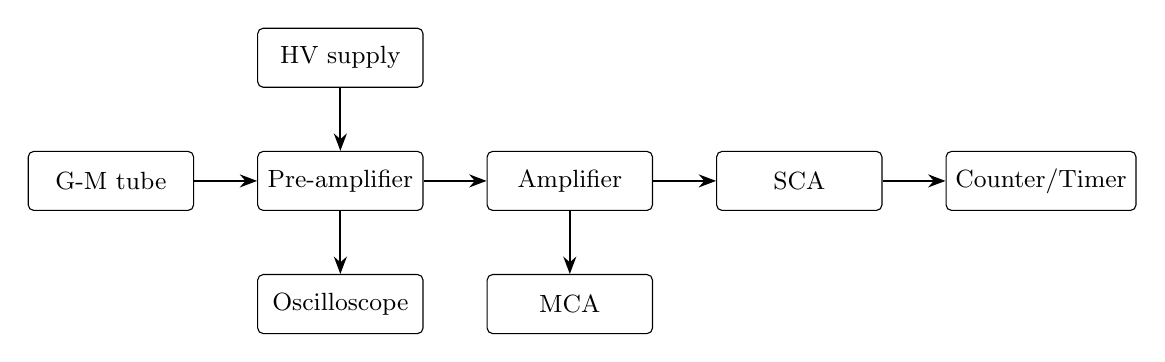
\begin{tikzpicture}[
    box/.style={draw, rounded corners=2pt, minimum width=2.1cm, minimum height=0.75cm, align=center, font=\small},
    arr/.style={-{Stealth[length=2.2mm]}, thick}
]
\node[box] (gm) {G-M tube};
\node[box, right=0.8cm of gm] (pre) {Pre-amplifier};
\node[box, right=0.8cm of pre] (amp) {Amplifier};
\node[box, right=0.8cm of amp] (sca) {SCA};
\node[box, right=0.8cm of sca] (ct) {Counter/Timer};
\node[box, above=0.8cm of pre] (hv) {HV supply};
\node[box, below=0.8cm of pre] (scope) {Oscilloscope};
\node[box, below=0.8cm of amp] (mca) {MCA};
\draw[arr] (gm) -- (pre);
\draw[arr] (hv) -- (pre);
\draw[arr] (pre) -- (amp);
\draw[arr] (amp) -- (sca);
\draw[arr] (sca) -- (ct);
\draw[arr] (pre) -- (scope);
\draw[arr] (amp) -- (mca);
\end{tikzpicture}
\caption{Block diagram of the setup.}
\label{fig:block}
\end{figure}

\subsection{Experimental Procedure}

We followed the lab manual \cite{labmanual} for all four measurements. The settings we had to find or choose are listed in Table \ref{tab:settings}.

\textbf{Counting curve and pulse height vs.\ HV.} With a source on the tube, we raised the high voltage from 650 V to 910 V in 20 V steps. At each step we waited 30 s for the voltage to settle, counted for 3 s with the counter/timer, and read the pre-amplifier pulse height on the oscilloscope. The pulse height uncertainty is the half width of the band of pulses, and the baseline correction is already applied to the tabulated values.  We took 840 V, on the high side of the plateau, as the operating voltage. The noise LLD (0.1 V) was found at 800 V with the source removed.

\textbf{Pulse height consistency.} At 840 V we recorded the pulse height spectra of Co-60, C-14 and Cl-36 with the MCA for 30 s real time each and took the centroid channel of the peak. We converted channels to volts with the calibration from our Lab 2 report \cite{lab2}.

\textbf{Beta attenuation.} We placed Al absorbers of increasing mass thickness between the Co-60 source and the tube, and counted for 5 to 14 s at each thickness (longer for thicker absorbers). The zero-absorber row in Table \ref{tab:rawbeta} is a background count.

\textbf{Dead time.} We measured the dead time and recovery time on the oscilloscope with the cursors on the persisting trace of the pulses, then used the two-source method with Th-232 and Cl-36. The sources sat on the 3rd shelf, about 3 cm from the tube and about 3 cm apart. A 1 mm change in position changes the rate noticeably, so the source that stays in place was never moved; only the other was inserted and removed. Each of the three runs has four 10 s counts: background, each source, and both together.

\begin{table}[!htbp]
\centering\small
\begin{tabular}{ll}
\toprule
\textbf{Setting} & \textbf{Value} \\
\midrule
High voltage scan & 650 to 910 V, 20 V steps, 30 s settle, 3 s count \\
Operating voltage & 840 V \\
Noise LLD & 0.1 V (found at 800 V, source removed) \\
SCA mode & integral \\
Scope baseline correction & $-2.625$ mV \\
Scope for dead time & 100 $\mu$s/div, Normal trigger, $\infty$ persist, trigger level $-78.2$ mV \\
MCA spectra & 30 s real time \\
Channel to voltage (Lab 2 \cite{lab2}) & $V = -36.0\ \text{mV} + (1.31\ \text{mV})\,n$, with $n$ the channel number \\
Two-source counts & 10 s each, 3rd shelf, sources about 3 cm from the tube \\
\bottomrule
\end{tabular}
\caption{Settings we found or chose.}
\label{tab:settings}
\end{table}


\section{Data}

\subsection{Counting curve and pulse height vs.\ high voltage}

Table \ref{tab:rawcc} lists the raw counts (3 s each) and the pre-amplifier pulse heights with their uncertainties. Counts first appeared at 670 V (44 counts), but no pulse was visible on the scope, so we attribute them to noise. Pulses first showed up on the scope at 690 V. At 910 V the counts jumped to 267 (177 at 890 V) and we stopped the scan.

\begin{table}[!htbp]
\centering\small\setlength{\tabcolsep}{3pt}
\begin{tabular}{ccc|ccc}
\toprule
\textbf{HV (V)} & \textbf{Counts (3 s)} & \textbf{Pulse height (mV)} & \textbf{HV (V)} & \textbf{Counts (3 s)} & \textbf{Pulse height (mV)} \\
\midrule
650 & 0 & 0 $\pm$ 0 & 790 & 169 & 137.5 $\pm$ 28.75 \\
670 & 44 & 0 $\pm$ 0 & 810 & 178 & 155.31 $\pm$ 29.06 \\
690 & 119 & 18.75 $\pm$ 2.75 & 830 & 183 & 212.81 $\pm$ 19.06 \\
710 & 152 & 31.125 $\pm$ 4.13 & 850 & 185 & 255 $\pm$ 21.25 \\
730 & 163 & 47.88 $\pm$ 9.13 & 870 & 178 & 303.75 $\pm$ 35 \\
750 & 164 & 70.5 $\pm$ 10.75 & 890 & 177 & 363.75 $\pm$ 52.5 \\
770 & 169 & 97.63 $\pm$ 14.38 & 910 & 267 & 443.75 $\pm$ 56.25 \\
\bottomrule
\end{tabular}
\caption{Counts in 3 s and pre-amplifier pulse height $\pm$ half width versus high voltage.}
\label{tab:rawcc}
\end{table}

\subsection{Pulse height consistency}

Table \ref{tab:rawcons} gives the MCA centroid channel and gross counts for each source.

\begin{table}[!htbp]
\centering\small
\begin{tabular}{lccc}
\toprule
\textbf{Source} & \textbf{Centroid channel} & \textbf{Gross counts} & \textbf{Real time (s)} \\
\midrule
Co-60 & 2906 & 4419 & 30 \\
C-14 & 3374 & 1280 & 30 \\
Cl-36 & 1939 & 13986 & 30 \\
\bottomrule
\end{tabular}
\caption{MCA centroid channel and gross counts for each source at 840 V.}
\label{tab:rawcons}
\end{table}

\todo[inline]{CELING: add the MCA spectra of Co-60, C-14 and Cl-36 here as Figure \ref{fig:mca} (placeholder).}
\begin{figure}[!htbp]
\centering
\fbox{\parbox{0.8\textwidth}{\centering\vspace{1.2cm}MCA spectra of Co-60, C-14 and Cl-36 (to be added)\vspace{1.2cm}}}
\caption{MCA pulse height spectra of the three sources at 840 V, 30 s real time.}
\label{fig:mca}
\end{figure}

\subsection{Beta attenuation}

Table \ref{tab:rawbeta} lists the absorber thickness, counts and counting time. The thickness uncertainty is 10\% of the thickness \cite{labmanual}.

\begin{table}[!htbp]
\centering\small
\begin{tabular}{lccc}
\toprule
\textbf{Absorber} & \textbf{Mass thickness (mg/cm$^2$)} & \textbf{Counts} & \textbf{Time (s)} \\
\midrule
Background (no source) & - & \multicolumn{1}{c}{5} & 5 \\
Al & 14.67 & 340 & 5 \\
Al & 66.53 & 83 & 5 \\
Al & 177.22 & 110 & 8 \\
Al & 415.80 & 112 & 8 \\
Al & 628.78 & 94 & 8 \\
Al & 843.34 & 139 & 12 \\
Al & 1278.61 & 84 & 14 \\
Al & 1540.52 & 100 & 14 \\
\bottomrule
\end{tabular}
\caption{Counts and counting time for each aluminum absorber with the Co-60 source.}
\label{tab:rawbeta}
\end{table}

\subsection{Dead time}

Figure \ref{fig:scope} shows the oscilloscope traces with the cursors placed as described in the manual \cite{labmanual}. The dead time runs from the initial pulse ($-2$ $\mu$s) to where pulses start to appear again (358 $\mu$s); the second measurement runs from there to where the pulses reach full height again (838 $\mu$s). The cursor step is 2 $\mu$s.

\begin{figure}[!htbp]
\centering
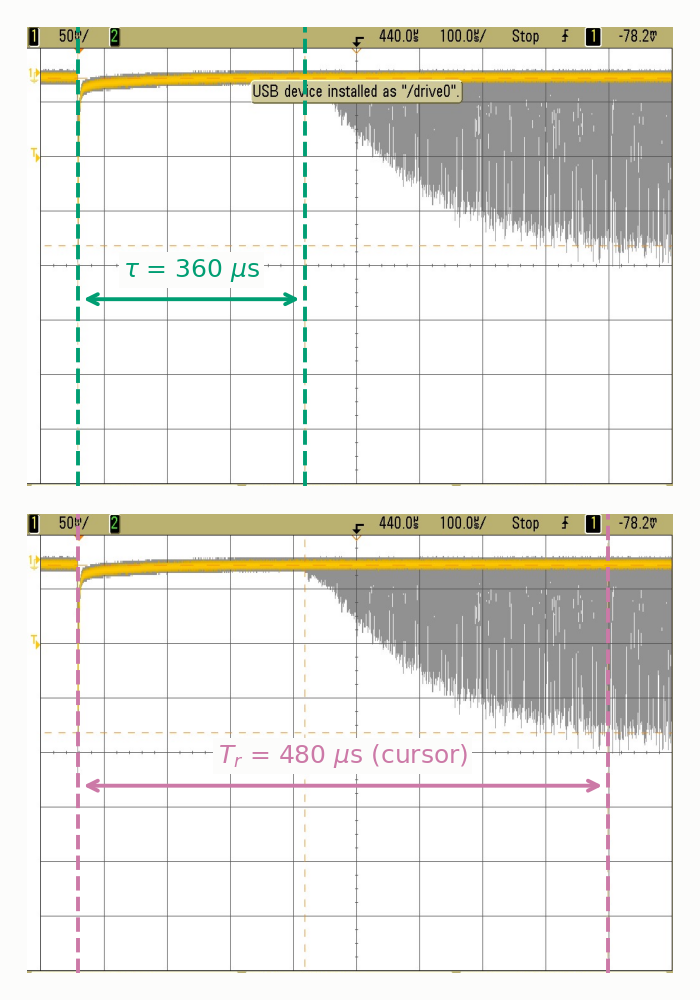
\includegraphics[width=0.36\textwidth]{figures/scope_cursors.png}
\caption{Oscilloscope traces with cursors: dead time (top, 360 $\mu$s) and recovery measurement (bottom, 480 $\mu$s).}
\label{fig:scope}
\end{figure}

Table \ref{tab:rawtwo} has the two-source counts.

\begin{table}[!htbp]
\centering\small
\begin{tabular}{ccccc}
\toprule
\textbf{Run} & \textbf{Background} & \textbf{Th-232} & \textbf{Cl-36} & \textbf{Both} \\
\midrule
1 & 5 & 1174 & 446 & 1585 \\
2 & 2 & 722 & 484 & 1163 \\
3 & 1 & 1056 & 441 & 1412 \\
\bottomrule
\end{tabular}
\caption{Two-source counts for each run (10 s per count).}
\label{tab:rawtwo}
\end{table}


\section{Analysis of Data}

Count uncertainties are Poisson, $\sigma_N = \sqrt{N}$, propagated with Knoll Eq.\ 3.37 and its special cases (Eqs.\ 3.38--3.42) \cite{knoll}. A rate from $N$ counts in time $t$ is $r = N/t$ with $\sigma_r = \sqrt{N}/t$ (Knoll, Eqs.\ 3.39--3.40).

\subsection{Counting curve and pulse height vs.\ high voltage}

\textbf{Count rates.} At 830 V we counted 183 in 3 s, so $r = 183/3 = \rEightThirty$ s$^{-1}$ and $\sigma_r = \sqrt{183}/3 = \srEightThirty$ s$^{-1}$. All rates are in Table \ref{tab:rate} and Figure \ref{fig:cc}b. The rates at the two voltages around the 840 V operating point are $\rEightThirty \pm \srEightThirty$ s$^{-1}$ (830 V) and $\rEightFifty \pm \srEightFifty$ s$^{-1}$ (850 V).

\begin{table}[!htbp]
\centering\small
\begin{tabular}{cc|cc}
\toprule
\textbf{HV (V)} & \textbf{Rate (s$^{-1}$)} & \textbf{HV (V)} & \textbf{Rate (s$^{-1}$)} \\
\midrule
650 & 0.0 $\pm$ 0.0 & 790 & 56.3 $\pm$ 4.3 \\
670 & 14.7 $\pm$ 2.2 & 810 & 59.3 $\pm$ 4.4 \\
690 & 39.7 $\pm$ 3.6 & 830 & 61.0 $\pm$ 4.5 \\
710 & 50.7 $\pm$ 4.1 & 850 & 61.7 $\pm$ 4.5 \\
730 & 54.3 $\pm$ 4.3 & 870 & 59.3 $\pm$ 4.4 \\
750 & 54.7 $\pm$ 4.3 & 890 & 59.0 $\pm$ 4.4 \\
770 & 56.3 $\pm$ 4.3 & 910 & 89.0 $\pm$ 5.4 \\
\bottomrule
\end{tabular}
\caption{Count rate $r = N/3$ s versus high voltage.}
\label{tab:rate}
\end{table}

\begin{figure}[!htbp]
\centering
\begin{subfigure}{0.46\textwidth}
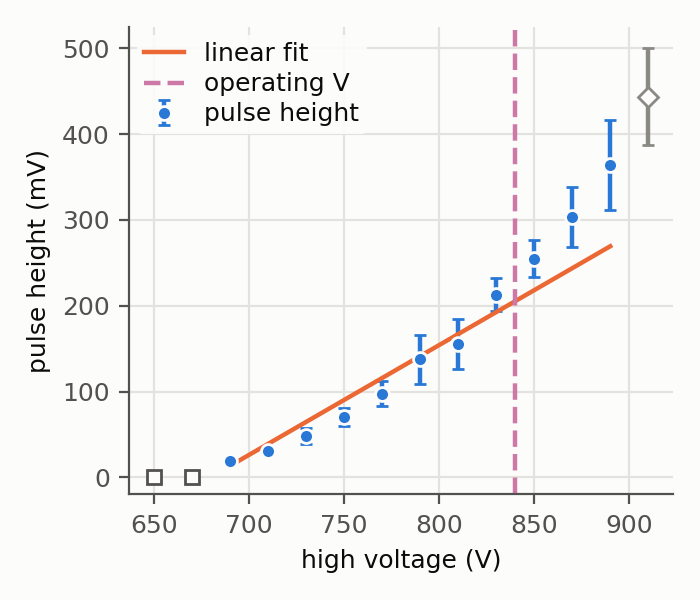
\includegraphics[width=\textwidth]{figures/pulse_height_vs_hv.png}
\caption{Pulse height}
\end{subfigure}
\hfill
\begin{subfigure}{0.46\textwidth}
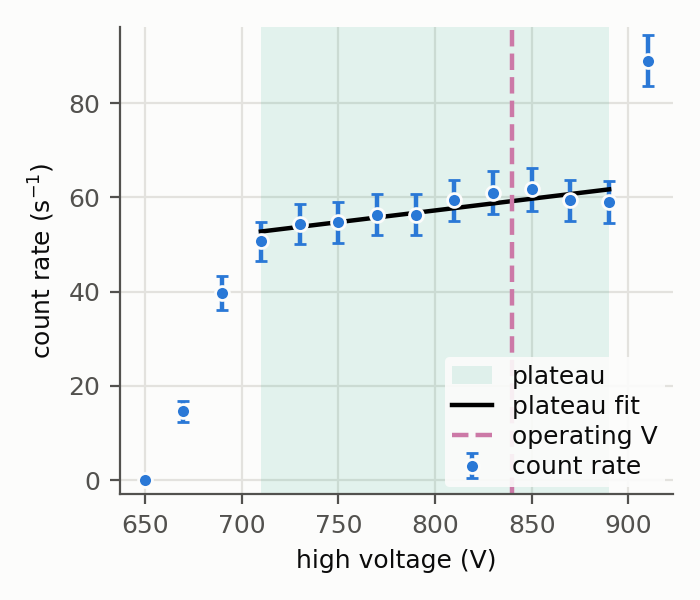
\includegraphics[width=\textwidth]{figures/counting_curve.png}
\caption{Counting curve}
\end{subfigure}
\caption{Pulse height (a) and count rate (b) versus high voltage. Dashed line: 840 V operating voltage. Error bars are the half width of the pulse band in (a) and $\sqrt{N}/t$ in (b).}
\label{fig:cc}
\end{figure}

\textbf{Plateau slope.} Knoll quotes the plateau slope in percent per 100 V (p.\ 215) \cite{knoll}. We take the plateau as 730--890 V and compare the mean rate of the three lowest points (730, 750, 770 V) with that of the three highest (850, 870, 890 V). A group rate is the summed counts over the summed time, with $\sigma = \sqrt{\sum N}/\sum t$ (Knoll, Eq.\ 3.42). Then
\begin{equation}
 s = \frac{r_2 - r_1}{V_2 - V_1}, \qquad
 \sigma_s = \frac{\sqrt{\sigma_{r_1}^2 + \sigma_{r_2}^2}}{V_2 - V_1}, \qquad
 s_{\%} = 100\,\frac{s\,(100\ \text{V})}{r_1},
\end{equation}
using Knoll Eq.\ 3.38 for $\sigma_s$ and the rate at the start of the plateau, $r_1$, as the reference rate. Sample calculation: $r_1 = \NoneA/9\ \text{s} = \rOneA \pm \srOneA$ s$^{-1}$ at $V_1 = 750$ V and $r_2 = \NtwoA/9\ \text{s} = \rTwoA \pm \srTwoA$ s$^{-1}$ at $V_2 = 870$ V, so
\[
 s = \frac{\rTwoA - \rOneA}{120\ \text{V}} = \pSlope \pm \spSlope\ \text{s}^{-1}\text{V}^{-1}, \qquad s_{\%} = \pPct \pm \spPct\ \%\ \text{per 100 V}.
\]

\todo[inline]{PARTNER: discuss the counting curve and pulse height vs.\ high voltage.}

\subsection{Pulse height consistency}

The Lab 2 calibration is channel $= 765.8\ \text{V} + 27.6$ \cite{lab2}, which we use as $V = -36.0\ \text{mV} + (1.31\ \text{mV})\,n$, with the Lab 2 oscilloscope amplitude uncertainty of 25.4 mV \cite{lab2}. For Co-60, $V = -36.0\ \text{mV} + 1.31\ \text{mV} \times \coCh = \coV$ V. The rate is $r = N/30$ s with $\sigma_r = \sqrt{N}/30$ s, so for Co-60 $r = \coG/30 = \coRate \pm \scoRate$ s$^{-1}$. Results are in Table \ref{tab:cons} and Figure \ref{fig:cons}.

\begin{table}[!htbp]
\centering\small
\begin{tabular}{lcc}
\toprule
\textbf{Source} & \textbf{Amplitude (V)} & \textbf{Rate (s$^{-1}$)} \\
\midrule
Co-60 & 3.77 $\pm$ 0.03 & 147 $\pm$ 2 \\
C-14 & 4.38 $\pm$ 0.03 & 43 $\pm$ 1 \\
Cl-36 & 2.50 $\pm$ 0.03 & 466 $\pm$ 4 \\
\bottomrule
\end{tabular}
\caption{Pulse amplitude (MCA centroid) and count rate at 840 V.}
\label{tab:cons}
\end{table}

\begin{figure}[!htbp]
\centering
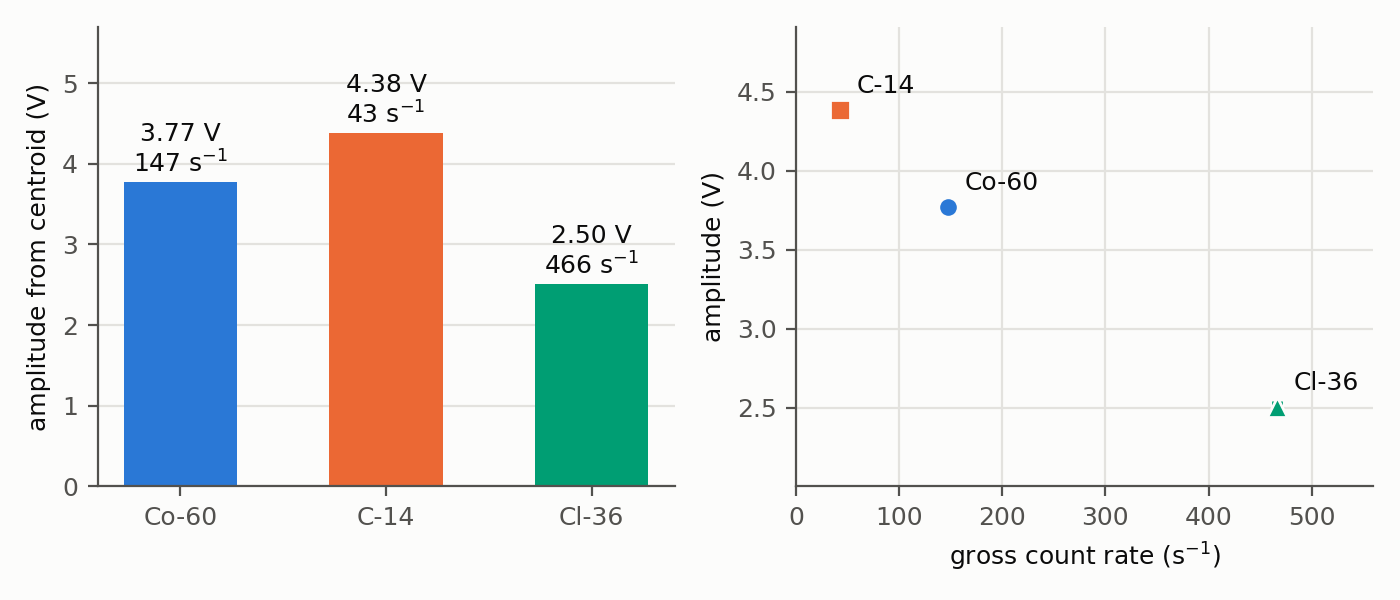
\includegraphics[width=0.85\textwidth]{figures/pulse_height_consistency.png}
\caption{Pulse amplitude from the MCA centroid and count rate for each source.}
\label{fig:cons}
\end{figure}

\todo[inline]{PARTNER: discuss the pulse height consistency.}

\subsection{Beta attenuation}

The net rate is the gross rate minus the background rate (Knoll, Eqs.\ 3.52--3.53) \cite{knoll},
\begin{equation}
 r = \frac{G}{t_g} - \frac{B}{t_b}, \qquad \sigma_r = \sqrt{\frac{G}{t_g^2} + \frac{B}{t_b^2}},
\end{equation}
with $G$, $t_g$ the gross counts and time and $B$, $t_b$ the background counts and time. The background is $B/t_b = 5/5 = \bkgR \pm \sbkgR$ s$^{-1}$. For 14.67 mg/cm$^2$: $G/t_g = 340/5 = \grossA \pm \sgrossA$ s$^{-1}$, so $r = \grossA - \bkgR = \netA \pm \snetA$ s$^{-1}$ and $\ln r = \lnA \pm \slnA$, using $\sigma_{\ln r} = \sigma_r/r$ (Knoll, Eq.\ 3.37). The thickness uncertainty is 10\% of the thickness \cite{labmanual}. Table \ref{tab:netbeta} and Figure \ref{fig:beta} show the results.

\begin{table}[!htbp]
\centering\small
\begin{tabular}{cccc}
\toprule
\textbf{Thickness (mg/cm$^2$)} & \textbf{Gross rate (s$^{-1}$)} & \textbf{Net rate (s$^{-1}$)} & \textbf{$\ln r$} \\
\midrule
14.7 & 68.00 $\pm$ 3.69 & 67.0 $\pm$ 3.7 & 4.20 $\pm$ 0.06 \\
66.5 & 16.60 $\pm$ 1.82 & 15.6 $\pm$ 1.9 & 2.75 $\pm$ 0.12 \\
177.2 & 13.75 $\pm$ 1.31 & 12.8 $\pm$ 1.4 & 2.55 $\pm$ 0.11 \\
415.8 & 14.00 $\pm$ 1.32 & 13.0 $\pm$ 1.4 & 2.56 $\pm$ 0.11 \\
628.8 & 11.75 $\pm$ 1.21 & 10.8 $\pm$ 1.3 & 2.37 $\pm$ 0.12 \\
843.3 & 11.58 $\pm$ 0.98 & 10.6 $\pm$ 1.1 & 2.36 $\pm$ 0.10 \\
1278.6 & 6.00 $\pm$ 0.65 & 5.0 $\pm$ 0.8 & 1.61 $\pm$ 0.16 \\
1540.5 & 7.14 $\pm$ 0.71 & 6.1 $\pm$ 0.8 & 1.82 $\pm$ 0.14 \\
\bottomrule
\end{tabular}
\caption{Gross rate, net rate and $\ln r$ for each absorber.}
\label{tab:netbeta}
\end{table}

\begin{figure}[!htbp]
\centering
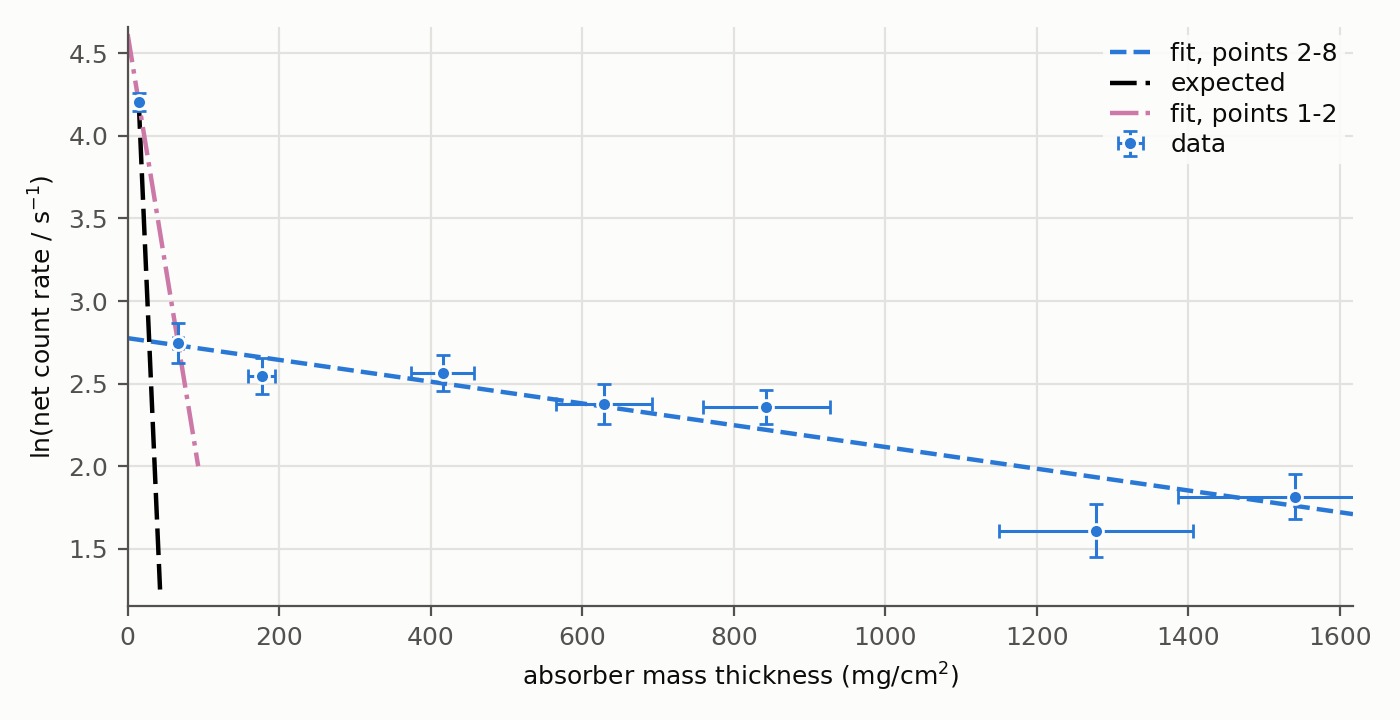
\includegraphics[width=0.75\textwidth]{figures/beta_attenuation_ln.png}
\caption{Natural log of the net count rate versus Al mass thickness. Dash-dot line: through points 1 and 2; dashed line: fit to points 2--8; black dashed line: expected $n$.}
\label{fig:beta}
\end{figure}

The beta count rate falls approximately as $I/I_0 = e^{-nt}$ with $t$ the mass thickness (Knoll, Eq.\ 2.14, p.\ 45) \cite{knoll}. We take $n$ from the first two points, since the rest of the data is nearly flat (Figure \ref{fig:beta}):
\begin{equation}
 n = \frac{\ln(r_1/r_2)}{t_2 - t_1}.
\end{equation}
The error follows from Knoll Eq.\ 3.37 with $\sigma_{r_1}$, $\sigma_{r_2}$ and the 10\% thickness uncertainties as independent inputs. With $\ln(\netA/\netB) = \lnRatio$ and $t_2 - t_1 = \dtAB$ g/cm$^2$,
\[
 n = \nTwo \pm \snTwo\ \text{cm}^2/\text{g}.
\]
We read the expected value for the Co-60 beta from Knoll Fig.\ 2.16 \cite{knoll}: $n_{\text{exp}} \approx \nExp \pm \snExp$ cm$^2$/g at the marked Co-60 endpoint energy ($\approx \EFig$ MeV). For the endpoint energy from our $n$ we inverted the line of Fig.\ 2.16, approximated by $E = 1.47\,(n/10)^{-0.668}$ MeV (our own reading of the log-log figure, not an equation from Knoll). This gives $E_{\max} = \EMeas \pm \sEMeas$ MeV (error from $\sigma_n$ only), and $\EExpFit$ MeV for $n_{\text{exp}}$.

\todo[inline]{PARTNER: discuss the beta attenuation (comparison with the expected $n$, endpoint energy).}

\subsection{Dead time}

\textbf{Oscilloscope.} The cursors in Figure \ref{fig:scope} give a dead time of $\sDead \pm \ssDead$ $\mu$s ($-2$ to 358 $\mu$s). The uncertainty is one cursor step (2 $\mu$s) on each cursor, added in quadrature. The interval from the end of the dead time to full pulse height is $\sInt \pm \ssDead$ $\mu$s (358 to 838 $\mu$s), and the recovery time measured from the initial pulse is $\sInit \pm \ssDead$ $\mu$s ($-2$ to 838 $\mu$s).

\textbf{Two-source method.} With background rate $m_b$, source rates $m_1$ (Th-232) and $m_2$ (Cl-36) and combined rate $m_{12}$, each the 10 s count divided by 10 s, the dead time of a non-paralyzable system is (Knoll, Eqs.\ 4.30--4.32) \cite{knoll}
\begin{align}
 X &= m_1 m_2 - m_b m_{12}, \qquad
 Y = m_1 m_2 (m_{12} + m_b) - m_b m_{12}(m_1 + m_2),\\
 Z &= \frac{Y\,(m_1 + m_2 - m_{12} - m_b)}{X^2}, \qquad
 \tau = \frac{X\left(1 - \sqrt{1 - Z}\right)}{Y}.
\end{align}
The uncertainty of $\tau$ is propagated with Knoll Eq.\ 3.37 from $\sigma_N = \sqrt{N}$ on the four counts. For run 1: $m_b = \sMb$, $m_1 = \sMone$, $m_2 = \sMtwo$ and $m_{12} = \sMonetwo$ s$^{-1}$ give $X = \sX$ s$^{-2}$, $Y = \sY$ s$^{-3}$, $Z = \sZ$, and $\tau = \sTau \pm \ssTau$ $\mu$s. The mean of the three runs and its standard error $s/\sqrt{3}$, with $s$ the sample standard deviation (Knoll, Eqs.\ 3.5, 3.9 and 3.37), are $\bar\tau = \tauMean \pm \tauSEM$ $\mu$s ($s = \tauSD$ $\mu$s). Table \ref{tab:tau} and Figure \ref{fig:tau} compare the runs with the oscilloscope dead time.

\begin{figure}[!htbp]
\centering
\begin{minipage}[c]{0.40\textwidth}\centering\small
\begin{tabular}{cc}
\toprule
\textbf{Run} & \textbf{$\tau$ ($\mu$s)} \\
\midrule
1 & 298 $\pm$ 566 \\
2 & 612 $\pm$ 729 \\
3 & 971 $\pm$ 634 \\
Mean $\pm$ SEM & 627 $\pm$ 195 \\
\bottomrule
\end{tabular}
\captionof{table}{Two-source dead time per run; SEM is the standard error of the mean.}
\label{tab:tau}
\end{minipage}\hfill
\begin{minipage}[c]{0.55\textwidth}\centering
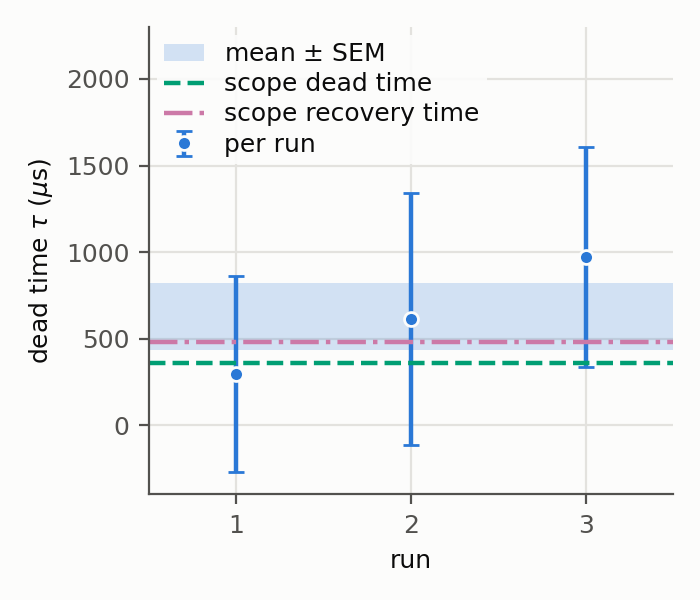
\includegraphics[width=\textwidth]{figures/dead_time_per_run.png}
\captionof{figure}{Two-source dead time per run, mean $\pm$ SEM, and the scope dead and recovery times.}
\label{fig:tau}
\end{minipage}
\end{figure}

\todo[inline]{PARTNER: discuss the two dead-time measurements (which to trust, the model assumed, recovery time).}


\section{Conclusions}

\todo[inline]{PARTNER writes this section.}

\nocite{knoll,labmanual,lab2} % remove once these are cited in the text
\bibliography{references}

\end{document}
